\documentclass{llncs}
%%%%%%%%%%%%%%%%%%%%%%
%%%%   PACKAGES   %%%%
%%%%%%%%%%%%%%%%%%%%%%
\usepackage{makeidx}
\usepackage{amsmath}
\usepackage{amssymb}
\usepackage{stmaryrd}
\usepackage{graphicx}
\usepackage{subfigure}
\usepackage{latexsym}
\usepackage{url}
\usepackage{color}
\usepackage{isabelle}
\usepackage{isabellesym}
\usepackage{theorem}
%\usepackage{times}
\usepackage{mathptmx}

%%%%%%%%%%%%%%%%%%%%%%%%%%%%
%For Isabelle code
\newlength{\fminilength}
\newsavebox{\fminibox}
\newenvironment{fmini}[1][\linewidth]
  {\setlength{\fminilength}{#1\fboxsep-2\fboxrule}%
   \vspace{2ex}\noindent\begin{lrbox}{\fminibox}\begin{minipage}{\fminilength}%
   \mbox{ }\hfill\vspace{-2.5ex}}%
  {\end{minipage}\end{lrbox}\vspace{1ex}\hspace{0ex}%
   \framebox{\usebox{\fminibox}}}

\newenvironment{specification}
{\noindent\footnotesize
\tt\begin{fmini}\begin{tabbing}X\=X12345\=XXXX\=XXXX\=XXXX\=XXXX\=XXXX
\=\+\kill} {\end{tabbing}\normalfont\end{fmini}}
\def \twoSpaces {\ \ }
%%%%%%%%%%%%%%%%%%%%%%%%%%%%

%%%%%%%%%%%%%%%%%%%%%%%%%%%%
%for comments
\newcommand\JP[1]{\textcolor{magenta}{JP: #1}}
\newcommand\lyj[1]{\textcolor{green}{lyj: #1}}
%%%%%%%%%%%%%%%%%%%%%%%%%%%

%%%%%%%%%%%%%%%%%%%%%%%%%%%
% Additional math operators
%%%%%%%%%%%%%%%%%%%%%%%%%%%

\usepackage[colorlinks,
            linkcolor=black,
            anchorcolor=black,
            citecolor=blue,
            urlcolor=black,
            bookmarks=true
            ]{hyperref}

% Macros for Scientific Word 2.5 documents saved with the LaTeX filter.
%Copyright (C) 1994-95 TCI Software Research, Inc.
\typeout{TCILATEX Macros for Scientific Word 2.5 <22 Dec 95>.}
\typeout{NOTICE:  This macro file is NOT proprietary and may be 
freely copied and distributed.}
%
\makeatletter
%
%%%%%%%%%%%%%%%%%%%%%%
% macros for time
\newcount\@hour\newcount\@minute\chardef\@x10\chardef\@xv60
\def\tcitime{
\def\@time{%
  \@minute\time\@hour\@minute\divide\@hour\@xv
  \ifnum\@hour<\@x 0\fi\the\@hour:%
  \multiply\@hour\@xv\advance\@minute-\@hour
  \ifnum\@minute<\@x 0\fi\the\@minute
  }}%

%%%%%%%%%%%%%%%%%%%%%%
% macro for hyperref
\@ifundefined{hyperref}{\def\hyperref#1#2#3#4{#2\ref{#4}#3}}{}

% macro for external program call
\@ifundefined{qExtProgCall}{\def\qExtProgCall#1#2#3#4#5#6{\relax}}{}
%%%%%%%%%%%%%%%%%%%%%%
%
% macros for graphics
%
\def\FILENAME#1{#1}%
%
\def\QCTOpt[#1]#2{%
  \def\QCTOptB{#1}
  \def\QCTOptA{#2}
}
\def\QCTNOpt#1{%
  \def\QCTOptA{#1}
  \let\QCTOptB\empty
}
\def\Qct{%
  \@ifnextchar[{%
    \QCTOpt}{\QCTNOpt}
}
\def\QCBOpt[#1]#2{%
  \def\QCBOptB{#1}
  \def\QCBOptA{#2}
}
\def\QCBNOpt#1{%
  \def\QCBOptA{#1}
  \let\QCBOptB\empty
}
\def\Qcb{%
  \@ifnextchar[{%
    \QCBOpt}{\QCBNOpt}
}
\def\PrepCapArgs{%
  \ifx\QCBOptA\empty
    \ifx\QCTOptA\empty
      {}%
    \else
      \ifx\QCTOptB\empty
        {\QCTOptA}%
      \else
        [\QCTOptB]{\QCTOptA}%
      \fi
    \fi
  \else
    \ifx\QCBOptA\empty
      {}%
    \else
      \ifx\QCBOptB\empty
        {\QCBOptA}%
      \else
        [\QCBOptB]{\QCBOptA}%
      \fi
    \fi
  \fi
}
\newcount\GRAPHICSTYPE
%\GRAPHICSTYPE 0 is for TurboTeX
%\GRAPHICSTYPE 1 is for DVIWindo (PostScript)
%%%(removed)%\GRAPHICSTYPE 2 is for psfig (PostScript)
\GRAPHICSTYPE=\z@
\def\GRAPHICSPS#1{%
 \ifcase\GRAPHICSTYPE%\GRAPHICSTYPE=0
   \special{ps: #1}%
 \or%\GRAPHICSTYPE=1
   \special{language "PS", include "#1"}%
%%%\or%\GRAPHICSTYPE=2
%%%  #1%
 \fi
}%
%
\def\GRAPHICSHP#1{\special{include #1}}%
%
% \graffile{ body }                                  %#1
%          { contentswidth (scalar)  }               %#2
%          { contentsheight (scalar) }               %#3
%          { vertical shift when in-line (scalar) }  %#4
\def\graffile#1#2#3#4{%
%%% \ifnum\GRAPHICSTYPE=\tw@
%%%  %Following if using psfig
%%%  \@ifundefined{psfig}{\input psfig.tex}{}%
%%%  \psfig{file=#1, height=#3, width=#2}%
%%% \else
  %Following for all others
  % JCS - added BOXTHEFRAME, see below
    \leavevmode
    \raise -#4 \BOXTHEFRAME{%
        \hbox to #2{\raise #3\hbox to #2{\null #1\hfil}}}%
}%
%
% A box for drafts
\def\draftbox#1#2#3#4{%
 \leavevmode\raise -#4 \hbox{%
  \frame{\rlap{\protect\tiny #1}\hbox to #2%
   {\vrule height#3 width\z@ depth\z@\hfil}%
  }%
 }%
}%
%
\newcount\draft
\draft=\z@
\let\nographics=\draft
\newif\ifwasdraft
\wasdraftfalse

%  \GRAPHIC{ body }                                  %#1
%          { draft name }                            %#2
%          { contentswidth (scalar)  }               %#3
%          { contentsheight (scalar) }               %#4
%          { vertical shift when in-line (scalar) }  %#5
\def\GRAPHIC#1#2#3#4#5{%
 \ifnum\draft=\@ne\draftbox{#2}{#3}{#4}{#5}%
  \else\graffile{#1}{#3}{#4}{#5}%
  \fi
 }%
%
\def\addtoLaTeXparams#1{%
    \edef\LaTeXparams{\LaTeXparams #1}}%
%
% JCS -  added a switch BoxFrame that can 
% be set by including X in the frame params.
% If set a box is drawn around the frame.

\newif\ifBoxFrame \BoxFramefalse
\newif\ifOverFrame \OverFramefalse
\newif\ifUnderFrame \UnderFramefalse

\def\BOXTHEFRAME#1{%
   \hbox{%
      \ifBoxFrame
         \frame{#1}%
      \else
         {#1}%
      \fi
   }%
}


\def\doFRAMEparams#1{\BoxFramefalse\OverFramefalse\UnderFramefalse\readFRAMEparams#1\end}%
\def\readFRAMEparams#1{%
 \ifx#1\end%
  \let\next=\relax
  \else
  \ifx#1i\dispkind=\z@\fi
  \ifx#1d\dispkind=\@ne\fi
  \ifx#1f\dispkind=\tw@\fi
  \ifx#1t\addtoLaTeXparams{t}\fi
  \ifx#1b\addtoLaTeXparams{b}\fi
  \ifx#1p\addtoLaTeXparams{p}\fi
  \ifx#1h\addtoLaTeXparams{h}\fi
  \ifx#1X\BoxFrametrue\fi
  \ifx#1O\OverFrametrue\fi
  \ifx#1U\UnderFrametrue\fi
  \ifx#1w
    \ifnum\draft=1\wasdrafttrue\else\wasdraftfalse\fi
    \draft=\@ne
  \fi
  \let\next=\readFRAMEparams
  \fi
 \next
 }%
%
%Macro for In-line graphics object
%   \IFRAME{ contentswidth (scalar)  }               %#1
%          { contentsheight (scalar) }               %#2
%          { vertical shift when in-line (scalar) }  %#3
%          { draft name }                            %#4
%          { body }                                  %#5
%          { caption}                                %#6


\def\IFRAME#1#2#3#4#5#6{%
      \bgroup
      \let\QCTOptA\empty
      \let\QCTOptB\empty
      \let\QCBOptA\empty
      \let\QCBOptB\empty
      #6%
      \parindent=0pt%
      \leftskip=0pt
      \rightskip=0pt
      \setbox0 = \hbox{\QCBOptA}%
      \@tempdima = #1\relax
      \ifOverFrame
          % Do this later
          \typeout{This is not implemented yet}%
          \show\HELP
      \else
         \ifdim\wd0>\@tempdima
            \advance\@tempdima by \@tempdima
            \ifdim\wd0 >\@tempdima
               \textwidth=\@tempdima
               \setbox1 =\vbox{%
                  \noindent\hbox to \@tempdima{\hfill\GRAPHIC{#5}{#4}{#1}{#2}{#3}\hfill}\\%
                  \noindent\hbox to \@tempdima{\parbox[b]{\@tempdima}{\QCBOptA}}%
               }%
               \wd1=\@tempdima
            \else
               \textwidth=\wd0
               \setbox1 =\vbox{%
                 \noindent\hbox to \wd0{\hfill\GRAPHIC{#5}{#4}{#1}{#2}{#3}\hfill}\\%
                 \noindent\hbox{\QCBOptA}%
               }%
               \wd1=\wd0
            \fi
         \else
            %\show\BBB
            \ifdim\wd0>0pt
              \hsize=\@tempdima
              \setbox1 =\vbox{%
                \unskip\GRAPHIC{#5}{#4}{#1}{#2}{0pt}%
                \break
                \unskip\hbox to \@tempdima{\hfill \QCBOptA\hfill}%
              }%
              \wd1=\@tempdima
           \else
              \hsize=\@tempdima
              \setbox1 =\vbox{%
                \unskip\GRAPHIC{#5}{#4}{#1}{#2}{0pt}%
              }%
              \wd1=\@tempdima
           \fi
         \fi
         \@tempdimb=\ht1
         \advance\@tempdimb by \dp1
         \advance\@tempdimb by -#2%
         \advance\@tempdimb by #3%
         \leavevmode
         \raise -\@tempdimb \hbox{\box1}%
      \fi
      \egroup%
}%
%
%Macro for Display graphics object
%   \DFRAME{ contentswidth (scalar)  }               %#1
%          { contentsheight (scalar) }               %#2
%          { draft label }                           %#3
%          { name }                                  %#4
%          { caption}                                %#5
\def\DFRAME#1#2#3#4#5{%
 \begin{center}
     \let\QCTOptA\empty
     \let\QCTOptB\empty
     \let\QCBOptA\empty
     \let\QCBOptB\empty
     \ifOverFrame 
        #5\QCTOptA\par
     \fi
     \GRAPHIC{#4}{#3}{#1}{#2}{\z@}
     \ifUnderFrame 
        \nobreak\par #5\QCBOptA
     \fi
 \end{center}%
 }%
%
%Macro for Floating graphic object
%   \FFRAME{ framedata f|i tbph x F|T }              %#1
%          { contentswidth (scalar)  }               %#2
%          { contentsheight (scalar) }               %#3
%          { caption }                               %#4
%          { label }                                 %#5
%          { draft name }                            %#6
%          { body }                                  %#7
\def\FFRAME#1#2#3#4#5#6#7{%
 \begin{figure}[#1]%
  \let\QCTOptA\empty
  \let\QCTOptB\empty
  \let\QCBOptA\empty
  \let\QCBOptB\empty
  \ifOverFrame
    #4
    \ifx\QCTOptA\empty
    \else
      \ifx\QCTOptB\empty
        \caption{\QCTOptA}%
      \else
        \caption[\QCTOptB]{\QCTOptA}%
      \fi
    \fi
    \ifUnderFrame\else
      \label{#5}%
    \fi
  \else
    \UnderFrametrue%
  \fi
  \begin{center}\GRAPHIC{#7}{#6}{#2}{#3}{\z@}\end{center}%
  \ifUnderFrame
    #4
    \ifx\QCBOptA\empty
      \caption{}%
    \else
      \ifx\QCBOptB\empty
        \caption{\QCBOptA}%
      \else
        \caption[\QCBOptB]{\QCBOptA}%
      \fi
    \fi
    \label{#5}%
  \fi
  \end{figure}%
 }%
%
%
%    \FRAME{ framedata f|i tbph x F|T }              %#1
%          { contentswidth (scalar)  }               %#2
%          { contentsheight (scalar) }               %#3
%          { vertical shift when in-line (scalar) }  %#4
%          { caption }                               %#5
%          { label }                                 %#6
%          { name }                                  %#7
%          { body }                                  %#8
%
%    framedata is a string which can contain the following
%    characters: idftbphxFT
%    Their meaning is as follows:
%             i, d or f : in-line, display, or floating
%             t,b,p,h   : LaTeX floating placement options
%             x         : fit contents box to contents
%             F or T    : Figure or Table. 
%                         Later this can expand
%                         to a more general float class.
%
%
\newcount\dispkind%

\def\makeactives{
  \catcode`\"=\active
  \catcode`\;=\active
  \catcode`\:=\active
  \catcode`\'=\active
  \catcode`\~=\active
}
\bgroup
   \makeactives
   \gdef\activesoff{%
      \def"{\string"}
      \def;{\string;}
      \def:{\string:}
      \def'{\string'}
      \def~{\string~}
      %\bbl@deactivate{"}%
      %\bbl@deactivate{;}%
      %\bbl@deactivate{:}%
      %\bbl@deactivate{'}%
    }
\egroup

\def\FRAME#1#2#3#4#5#6#7#8{%
 \bgroup
 \@ifundefined{bbl@deactivate}{}{\activesoff}
 \ifnum\draft=\@ne
   \wasdrafttrue
 \else
   \wasdraftfalse%
 \fi
 \def\LaTeXparams{}%
 \dispkind=\z@
 \def\LaTeXparams{}%
 \doFRAMEparams{#1}%
 \ifnum\dispkind=\z@\IFRAME{#2}{#3}{#4}{#7}{#8}{#5}\else
  \ifnum\dispkind=\@ne\DFRAME{#2}{#3}{#7}{#8}{#5}\else
   \ifnum\dispkind=\tw@
    \edef\@tempa{\noexpand\FFRAME{\LaTeXparams}}%
    \@tempa{#2}{#3}{#5}{#6}{#7}{#8}%
    \fi
   \fi
  \fi
  \ifwasdraft\draft=1\else\draft=0\fi{}%
  \egroup
 }%
%
% This macro added to let SW gobble a parameter that
% should not be passed on and expanded. 

\def\TEXUX#1{"texux"}

%
% Macros for text attributes:
%
\def\BF#1{{\bf {#1}}}%
\def\NEG#1{\leavevmode\hbox{\rlap{\thinspace/}{$#1$}}}%
%
%%%%%%%%%%%%%%%%%%%%%%%%%%%%%%%%%%%%%%%%%%%%%%%%%%%%%%%%%%%%%%%%%%%%%%%%
%
%
% macros for user - defined functions
\def\func#1{\mathop{\rm #1}}%
\def\limfunc#1{\mathop{\rm #1}}%

%
% miscellaneous 
%\long\def\QQQ#1#2{}%
\long\def\QQQ#1#2{%
     \long\expandafter\def\csname#1\endcsname{#2}}%
%\def\QTP#1{}% JCS - this was changed becuase style editor will define QTP
\@ifundefined{QTP}{\def\QTP#1{}}{}
\@ifundefined{QEXCLUDE}{\def\QEXCLUDE#1{}}{}
%\@ifundefined{Qcb}{\def\Qcb#1{#1}}{}
%\@ifundefined{Qct}{\def\Qct#1{#1}}{}
\@ifundefined{Qlb}{\def\Qlb#1{#1}}{}
\@ifundefined{Qlt}{\def\Qlt#1{#1}}{}
\def\QWE{}%
\long\def\QQA#1#2{}%
%\def\QTR#1#2{{\em #2}}% Always \em!!!
%\def\QTR#1#2{\mbox{\begin{#1}#2\end{#1}}}%cb%%%
\def\QTR#1#2{{\csname#1\endcsname #2}}%(gp) Is this the best?
\long\def\TeXButton#1#2{#2}%
\long\def\QSubDoc#1#2{#2}%
\def\EXPAND#1[#2]#3{}%
\def\NOEXPAND#1[#2]#3{}%
\def\PROTECTED{}%
\def\LaTeXparent#1{}%
\def\ChildStyles#1{}%
\def\ChildDefaults#1{}%
\def\QTagDef#1#2#3{}%
%
% Macros for style editor docs
\@ifundefined{StyleEditBeginDoc}{\def\StyleEditBeginDoc{\relax}}{}
%
% Macros for footnotes
\def\QQfnmark#1{\footnotemark}
\def\QQfntext#1#2{\addtocounter{footnote}{#1}\footnotetext{#2}}
%
% Macros for indexing.
\def\MAKEINDEX{\makeatletter\input gnuindex.sty\makeatother\makeindex}%	
\@ifundefined{INDEX}{\def\INDEX#1#2{}{}}{}%
\@ifundefined{SUBINDEX}{\def\SUBINDEX#1#2#3{}{}{}}{}%
\@ifundefined{initial}%  
   {\def\initial#1{\bigbreak{\raggedright\large\bf #1}\kern 2\p@\penalty3000}}%
   {}%
\@ifundefined{entry}{\def\entry#1#2{\item {#1}, #2}}{}%
\@ifundefined{primary}{\def\primary#1{\item {#1}}}{}%
\@ifundefined{secondary}{\def\secondary#1#2{\subitem {#1}, #2}}{}%
%
%
\@ifundefined{ZZZ}{}{\MAKEINDEX\makeatletter}%
%
% Attempts to avoid problems with other styles
\@ifundefined{abstract}{%
 \def\abstract{%
  \if@twocolumn
   \section*{Abstract (Not appropriate in this style!)}%
   \else \small 
   \begin{center}{\bf Abstract\vspace{-.5em}\vspace{\z@}}\end{center}%
   \quotation 
   \fi
  }%
 }{%
 }%
\@ifundefined{endabstract}{\def\endabstract
  {\if@twocolumn\else\endquotation\fi}}{}%
\@ifundefined{maketitle}{\def\maketitle#1{}}{}%
\@ifundefined{affiliation}{\def\affiliation#1{}}{}%
\@ifundefined{proof}{\def\proof{\noindent{\bfseries Proof. }}}{}%
\@ifundefined{endproof}{\def\endproof{\mbox{\ \rule{.1in}{.1in}}}}{}%
\@ifundefined{newfield}{\def\newfield#1#2{}}{}%
\@ifundefined{chapter}{\def\chapter#1{\par(Chapter head:)#1\par }%
 \newcount\c@chapter}{}%
\@ifundefined{part}{\def\part#1{\par(Part head:)#1\par }}{}%
\@ifundefined{section}{\def\section#1{\par(Section head:)#1\par }}{}%
\@ifundefined{subsection}{\def\subsection#1%
 {\par(Subsection head:)#1\par }}{}%
\@ifundefined{subsubsection}{\def\subsubsection#1%
 {\par(Subsubsection head:)#1\par }}{}%
\@ifundefined{paragraph}{\def\paragraph#1%
 {\par(Subsubsubsection head:)#1\par }}{}%
\@ifundefined{subparagraph}{\def\subparagraph#1%
 {\par(Subsubsubsubsection head:)#1\par }}{}%
%%%%%%%%%%%%%%%%%%%%%%%%%%%%%%%%%%%%%%%%%%%%%%%%%%%%%%%%%%%%%%%%%%%%%%%%
% These symbols are not recognized by LaTeX
\@ifundefined{therefore}{\def\therefore{}}{}%
\@ifundefined{backepsilon}{\def\backepsilon{}}{}%
\@ifundefined{yen}{\def\yen{\hbox{\rm\rlap=Y}}}{}%
\@ifundefined{registered}{%
   \def\registered{\relax\ifmmode{}\r@gistered
                    \else$\m@th\r@gistered$\fi}%
 \def\r@gistered{^{\ooalign
  {\hfil\raise.07ex\hbox{$\scriptstyle\rm\text{R}$}\hfil\crcr
  \mathhexbox20D}}}}{}%
\@ifundefined{Eth}{\def\Eth{}}{}%
\@ifundefined{eth}{\def\eth{}}{}%
\@ifundefined{Thorn}{\def\Thorn{}}{}%
\@ifundefined{thorn}{\def\thorn{}}{}%
% A macro to allow any symbol that requires math to appear in text
\def\TEXTsymbol#1{\mbox{$#1$}}%
\@ifundefined{degree}{\def\degree{{}^{\circ}}}{}%
%
% macros for T3TeX files
\newdimen\theight
\def\Column{%
 \vadjust{\setbox\z@=\hbox{\scriptsize\quad\quad tcol}%
  \theight=\ht\z@\advance\theight by \dp\z@\advance\theight by \lineskip
  \kern -\theight \vbox to \theight{%
   \rightline{\rlap{\box\z@}}%
   \vss
   }%
  }%
 }%
%
\def\qed{%
 \ifhmode\unskip\nobreak\fi\ifmmode\ifinner\else\hskip5\p@\fi\fi
 \hbox{\hskip5\p@\vrule width4\p@ height6\p@ depth1.5\p@\hskip\p@}%
 }%
%
\def\cents{\hbox{\rm\rlap/c}}%
\def\miss{\hbox{\vrule height2\p@ width 2\p@ depth\z@}}%
%\def\miss{\hbox{.}}%        %another possibility 
%
\def\vvert{\Vert}%           %always translated to \left| or \right|
%
\def\tcol#1{{\baselineskip=6\p@ \vcenter{#1}} \Column}  %
%
\def\dB{\hbox{{}}}%                 %dummy entry in column 
\def\mB#1{\hbox{$#1$}}%             %column entry
\def\nB#1{\hbox{#1}}%               %column entry (not math)
%
%\newcount\notenumber
%\def\clearnotenumber{\notenumber=0}
%\def\note{\global\advance\notenumber by 1
% \footnote{$^{\the\notenumber}$}}
%\def\note{\global\advance\notenumber by 1
\def\note{$^{\dag}}%
%
%

\def\newfmtname{LaTeX2e}
\def\chkcompat{%
   \if@compatibility
   \else
     \usepackage{latexsym}
   \fi
}

\ifx\fmtname\newfmtname
  \DeclareOldFontCommand{\rm}{\normalfont\rmfamily}{\mathrm}
  \DeclareOldFontCommand{\sf}{\normalfont\sffamily}{\mathsf}
  \DeclareOldFontCommand{\tt}{\normalfont\ttfamily}{\mathtt}
  \DeclareOldFontCommand{\bf}{\normalfont\bfseries}{\mathbf}
  \DeclareOldFontCommand{\it}{\normalfont\itshape}{\mathit}
  \DeclareOldFontCommand{\sl}{\normalfont\slshape}{\@nomath\sl}
  \DeclareOldFontCommand{\sc}{\normalfont\scshape}{\@nomath\sc}
  \chkcompat
\fi

%
% Greek bold macros
% Redefine all of the math symbols 
% which might be bolded	 - there are 
% probably others to add to this list

\def\alpha{\Greekmath 010B }%
\def\beta{\Greekmath 010C }%
\def\gamma{\Greekmath 010D }%
\def\delta{\Greekmath 010E }%
\def\epsilon{\Greekmath 010F }%
\def\zeta{\Greekmath 0110 }%
\def\eta{\Greekmath 0111 }%
\def\theta{\Greekmath 0112 }%
\def\iota{\Greekmath 0113 }%
\def\kappa{\Greekmath 0114 }%
\def\lambda{\Greekmath 0115 }%
\def\mu{\Greekmath 0116 }%
\def\nu{\Greekmath 0117 }%
\def\xi{\Greekmath 0118 }%
\def\pi{\Greekmath 0119 }%
\def\rho{\Greekmath 011A }%
\def\sigma{\Greekmath 011B }%
\def\tau{\Greekmath 011C }%
\def\upsilon{\Greekmath 011D }%
\def\phi{\Greekmath 011E }%
\def\chi{\Greekmath 011F }%
\def\psi{\Greekmath 0120 }%
\def\omega{\Greekmath 0121 }%
\def\varepsilon{\Greekmath 0122 }%
\def\vartheta{\Greekmath 0123 }%
\def\varpi{\Greekmath 0124 }%
\def\varrho{\Greekmath 0125 }%
\def\varsigma{\Greekmath 0126 }%
\def\varphi{\Greekmath 0127 }%

\def\nabla{\Greekmath 0272 }
\def\FindBoldGroup{%
   {\setbox0=\hbox{$\mathbf{x\global\edef\theboldgroup{\the\mathgroup}}$}}%
}

\def\Greekmath#1#2#3#4{%
    \if@compatibility
        \ifnum\mathgroup=\symbold
           \mathchoice{\mbox{\boldmath$\displaystyle\mathchar"#1#2#3#4$}}%
                      {\mbox{\boldmath$\textstyle\mathchar"#1#2#3#4$}}%
                      {\mbox{\boldmath$\scriptstyle\mathchar"#1#2#3#4$}}%
                      {\mbox{\boldmath$\scriptscriptstyle\mathchar"#1#2#3#4$}}%
        \else
           \mathchar"#1#2#3#4% 
        \fi 
    \else 
        \FindBoldGroup
        \ifnum\mathgroup=\theboldgroup % For 2e
           \mathchoice{\mbox{\boldmath$\displaystyle\mathchar"#1#2#3#4$}}%
                      {\mbox{\boldmath$\textstyle\mathchar"#1#2#3#4$}}%
                      {\mbox{\boldmath$\scriptstyle\mathchar"#1#2#3#4$}}%
                      {\mbox{\boldmath$\scriptscriptstyle\mathchar"#1#2#3#4$}}%
        \else
           \mathchar"#1#2#3#4% 
        \fi     	    
	  \fi}

\newif\ifGreekBold  \GreekBoldfalse
\let\SAVEPBF=\pbf
\def\pbf{\GreekBoldtrue\SAVEPBF}%
%

\@ifundefined{theorem}{\newtheorem{theorem}{Theorem}}{}
\@ifundefined{lemma}{\newtheorem{lemma}[theorem]{Lemma}}{}
\@ifundefined{corollary}{\newtheorem{corollary}[theorem]{Corollary}}{}
\@ifundefined{conjecture}{\newtheorem{conjecture}[theorem]{Conjecture}}{}
\@ifundefined{proposition}{\newtheorem{proposition}[theorem]{Proposition}}{}
\@ifundefined{axiom}{\newtheorem{axiom}{Axiom}}{}
\@ifundefined{remark}{\newtheorem{remark}{Remark}}{}
\@ifundefined{example}{\newtheorem{example}{Example}}{}
\@ifundefined{exercise}{\newtheorem{exercise}{Exercise}}{}
\@ifundefined{definition}{\newtheorem{definition}{Definition}}{}


\@ifundefined{mathletters}{%
  %\def\theequation{\arabic{equation}}
  \newcounter{equationnumber}  
  \def\mathletters{%
     \addtocounter{equation}{1}
     \edef\@currentlabel{\theequation}%
     \setcounter{equationnumber}{\c@equation}
     \setcounter{equation}{0}%
     \edef\theequation{\@currentlabel\noexpand\alph{equation}}%
  }
  \def\endmathletters{%
     \setcounter{equation}{\value{equationnumber}}%
  }
}{}

%Logos
\@ifundefined{BibTeX}{%
    \def\BibTeX{{\rm B\kern-.05em{\sc i\kern-.025em b}\kern-.08em
                 T\kern-.1667em\lower.7ex\hbox{E}\kern-.125emX}}}{}%
\@ifundefined{AmS}%
    {\def\AmS{{\protect\usefont{OMS}{cmsy}{m}{n}%
                A\kern-.1667em\lower.5ex\hbox{M}\kern-.125emS}}}{}%
\@ifundefined{AmSTeX}{\def\AmSTeX{\protect\AmS-\protect\TeX\@}}{}%
%

%%%%%%%%%%%%%%%%%%%%%%%%%%%%%%%%%%%%%%%%%%%%%%%%%%%%%%%%%%%%%%%%%%%%%%%
% NOTE: The rest of this file is read only if amstex has not been
% loaded.  This section is used to define amstex constructs in the
% event they have not been defined.
%
%
\ifx\ds@amstex\relax
   \message{amstex already loaded}\makeatother\endinput% 2.09 compatability
\else
   \@ifpackageloaded{amstex}%
      {\message{amstex already loaded}\makeatother\endinput}
      {}
   \@ifpackageloaded{amsgen}%
      {\message{amsgen already loaded}\makeatother\endinput}
      {}
\fi
%%%%%%%%%%%%%%%%%%%%%%%%%%%%%%%%%%%%%%%%%%%%%%%%%%%%%%%%%%%%%%%%%%%%%%%%
%%
%
%
%  Macros to define some AMS LaTeX constructs when 
%  AMS LaTeX has not been loaded
% 
% These macros are copied from the AMS-TeX package for doing
% multiple integrals.
%
\let\DOTSI\relax
\def\RIfM@{\relax\ifmmode}%
\def\FN@{\futurelet\next}%
\newcount\intno@
\def\iint{\DOTSI\intno@\tw@\FN@\ints@}%
\def\iiint{\DOTSI\intno@\thr@@\FN@\ints@}%
\def\iiiint{\DOTSI\intno@4 \FN@\ints@}%
\def\idotsint{\DOTSI\intno@\z@\FN@\ints@}%
\def\ints@{\findlimits@\ints@@}%
\newif\iflimtoken@
\newif\iflimits@
\def\findlimits@{\limtoken@true\ifx\next\limits\limits@true
 \else\ifx\next\nolimits\limits@false\else
 \limtoken@false\ifx\ilimits@\nolimits\limits@false\else
 \ifinner\limits@false\else\limits@true\fi\fi\fi\fi}%
\def\multint@{\int\ifnum\intno@=\z@\intdots@                          %1
 \else\intkern@\fi                                                    %2
 \ifnum\intno@>\tw@\int\intkern@\fi                                   %3
 \ifnum\intno@>\thr@@\int\intkern@\fi                                 %4
 \int}%                                                               %5
\def\multintlimits@{\intop\ifnum\intno@=\z@\intdots@\else\intkern@\fi
 \ifnum\intno@>\tw@\intop\intkern@\fi
 \ifnum\intno@>\thr@@\intop\intkern@\fi\intop}%
\def\intic@{%
    \mathchoice{\hskip.5em}{\hskip.4em}{\hskip.4em}{\hskip.4em}}%
\def\negintic@{\mathchoice
 {\hskip-.5em}{\hskip-.4em}{\hskip-.4em}{\hskip-.4em}}%
\def\ints@@{\iflimtoken@                                              %1
 \def\ints@@@{\iflimits@\negintic@
   \mathop{\intic@\multintlimits@}\limits                             %2
  \else\multint@\nolimits\fi                                          %3
  \eat@}%                                                             %4
 \else                                                                %5
 \def\ints@@@{\iflimits@\negintic@
  \mathop{\intic@\multintlimits@}\limits\else
  \multint@\nolimits\fi}\fi\ints@@@}%
\def\intkern@{\mathchoice{\!\!\!}{\!\!}{\!\!}{\!\!}}%
\def\plaincdots@{\mathinner{\cdotp\cdotp\cdotp}}%
\def\intdots@{\mathchoice{\plaincdots@}%
 {{\cdotp}\mkern1.5mu{\cdotp}\mkern1.5mu{\cdotp}}%
 {{\cdotp}\mkern1mu{\cdotp}\mkern1mu{\cdotp}}%
 {{\cdotp}\mkern1mu{\cdotp}\mkern1mu{\cdotp}}}%
%
%
%  These macros are for doing the AMS \text{} construct
%
\def\RIfM@{\relax\protect\ifmmode}
\def\text{\RIfM@\expandafter\text@\else\expandafter\mbox\fi}
\let\nfss@text\text
\def\text@#1{\mathchoice
   {\textdef@\displaystyle\f@size{#1}}%
   {\textdef@\textstyle\tf@size{\firstchoice@false #1}}%
   {\textdef@\textstyle\sf@size{\firstchoice@false #1}}%
   {\textdef@\textstyle \ssf@size{\firstchoice@false #1}}%
   \glb@settings}

\def\textdef@#1#2#3{\hbox{{%
                    \everymath{#1}%
                    \let\f@size#2\selectfont
                    #3}}}
\newif\iffirstchoice@
\firstchoice@true
%
%    Old Scheme for \text
%
%\def\rmfam{\z@}%
%\newif\iffirstchoice@
%\firstchoice@true
%\def\textfonti{\the\textfont\@ne}%
%\def\textfontii{\the\textfont\tw@}%
%\def\text{\RIfM@\expandafter\text@\else\expandafter\text@@\fi}%
%\def\text@@#1{\leavevmode\hbox{#1}}%
%\def\text@#1{\mathchoice
% {\hbox{\everymath{\displaystyle}\def\textfonti{\the\textfont\@ne}%
%  \def\textfontii{\the\textfont\tw@}\textdef@@ T#1}}%
% {\hbox{\firstchoice@false
%  \everymath{\textstyle}\def\textfonti{\the\textfont\@ne}%
%  \def\textfontii{\the\textfont\tw@}\textdef@@ T#1}}%
% {\hbox{\firstchoice@false
%  \everymath{\scriptstyle}\def\textfonti{\the\scriptfont\@ne}%
%  \def\textfontii{\the\scriptfont\tw@}\textdef@@ S\rm#1}}%
% {\hbox{\firstchoice@false
%  \everymath{\scriptscriptstyle}\def\textfonti
%  {\the\scriptscriptfont\@ne}%
%  \def\textfontii{\the\scriptscriptfont\tw@}\textdef@@ s\rm#1}}}%
%\def\textdef@@#1{\textdef@#1\rm\textdef@#1\bf\textdef@#1\sl
%    \textdef@#1\it}%
%\def\DN@{\def\next@}%
%\def\eat@#1{}%
%\def\textdef@#1#2{%
% \DN@{\csname\expandafter\eat@\string#2fam\endcsname}%
% \if S#1\edef#2{\the\scriptfont\next@\relax}%
% \else\if s#1\edef#2{\the\scriptscriptfont\next@\relax}%
% \else\edef#2{\the\textfont\next@\relax}\fi\fi}%
%
%
%These are the AMS constructs for multiline limits.
%
\def\Let@{\relax\iffalse{\fi\let\\=\cr\iffalse}\fi}%
\def\vspace@{\def\vspace##1{\crcr\noalign{\vskip##1\relax}}}%
\def\multilimits@{\bgroup\vspace@\Let@
 \baselineskip\fontdimen10 \scriptfont\tw@
 \advance\baselineskip\fontdimen12 \scriptfont\tw@
 \lineskip\thr@@\fontdimen8 \scriptfont\thr@@
 \lineskiplimit\lineskip
 \vbox\bgroup\ialign\bgroup\hfil$\m@th\scriptstyle{##}$\hfil\crcr}%
\def\Sb{_\multilimits@}%
\def\endSb{\crcr\egroup\egroup\egroup}%
\def\Sp{^\multilimits@}%
\let\endSp\endSb
%
%
%These are AMS constructs for horizontal arrows
%
\newdimen\ex@
\ex@.2326ex
\def\rightarrowfill@#1{$#1\m@th\mathord-\mkern-6mu\cleaders
 \hbox{$#1\mkern-2mu\mathord-\mkern-2mu$}\hfill
 \mkern-6mu\mathord\rightarrow$}%
\def\leftarrowfill@#1{$#1\m@th\mathord\leftarrow\mkern-6mu\cleaders
 \hbox{$#1\mkern-2mu\mathord-\mkern-2mu$}\hfill\mkern-6mu\mathord-$}%
\def\leftrightarrowfill@#1{$#1\m@th\mathord\leftarrow
\mkern-6mu\cleaders
 \hbox{$#1\mkern-2mu\mathord-\mkern-2mu$}\hfill
 \mkern-6mu\mathord\rightarrow$}%
\def\overrightarrow{\mathpalette\overrightarrow@}%
\def\overrightarrow@#1#2{\vbox{\ialign{##\crcr\rightarrowfill@#1\crcr
 \noalign{\kern-\ex@\nointerlineskip}$\m@th\hfil#1#2\hfil$\crcr}}}%
\let\overarrow\overrightarrow
\def\overleftarrow{\mathpalette\overleftarrow@}%
\def\overleftarrow@#1#2{\vbox{\ialign{##\crcr\leftarrowfill@#1\crcr
 \noalign{\kern-\ex@\nointerlineskip}$\m@th\hfil#1#2\hfil$\crcr}}}%
\def\overleftrightarrow{\mathpalette\overleftrightarrow@}%
\def\overleftrightarrow@#1#2{\vbox{\ialign{##\crcr
   \leftrightarrowfill@#1\crcr
 \noalign{\kern-\ex@\nointerlineskip}$\m@th\hfil#1#2\hfil$\crcr}}}%
\def\underrightarrow{\mathpalette\underrightarrow@}%
\def\underrightarrow@#1#2{\vtop{\ialign{##\crcr$\m@th\hfil#1#2\hfil
  $\crcr\noalign{\nointerlineskip}\rightarrowfill@#1\crcr}}}%
\let\underarrow\underrightarrow
\def\underleftarrow{\mathpalette\underleftarrow@}%
\def\underleftarrow@#1#2{\vtop{\ialign{##\crcr$\m@th\hfil#1#2\hfil
  $\crcr\noalign{\nointerlineskip}\leftarrowfill@#1\crcr}}}%
\def\underleftrightarrow{\mathpalette\underleftrightarrow@}%
\def\underleftrightarrow@#1#2{\vtop{\ialign{##\crcr$\m@th
  \hfil#1#2\hfil$\crcr
 \noalign{\nointerlineskip}\leftrightarrowfill@#1\crcr}}}%
%%%%%%%%%%%%%%%%%%%%%

% 94.0815 by Jon:

\def\qopnamewl@#1{\mathop{\operator@font#1}\nlimits@}
\let\nlimits@\displaylimits
\def\setboxz@h{\setbox\z@\hbox}


\def\varlim@#1#2{\mathop{\vtop{\ialign{##\crcr
 \hfil$#1\m@th\operator@font lim$\hfil\crcr
 \noalign{\nointerlineskip}#2#1\crcr
 \noalign{\nointerlineskip\kern-\ex@}\crcr}}}}

 \def\rightarrowfill@#1{\m@th\setboxz@h{$#1-$}\ht\z@\z@
  $#1\copy\z@\mkern-6mu\cleaders
  \hbox{$#1\mkern-2mu\box\z@\mkern-2mu$}\hfill
  \mkern-6mu\mathord\rightarrow$}
\def\leftarrowfill@#1{\m@th\setboxz@h{$#1-$}\ht\z@\z@
  $#1\mathord\leftarrow\mkern-6mu\cleaders
  \hbox{$#1\mkern-2mu\copy\z@\mkern-2mu$}\hfill
  \mkern-6mu\box\z@$}


\def\projlim{\qopnamewl@{proj\,lim}}
\def\injlim{\qopnamewl@{inj\,lim}}
\def\varinjlim{\mathpalette\varlim@\rightarrowfill@}
\def\varprojlim{\mathpalette\varlim@\leftarrowfill@}
\def\varliminf{\mathpalette\varliminf@{}}
\def\varliminf@#1{\mathop{\underline{\vrule\@depth.2\ex@\@width\z@
   \hbox{$#1\m@th\operator@font lim$}}}}
\def\varlimsup{\mathpalette\varlimsup@{}}
\def\varlimsup@#1{\mathop{\overline
  {\hbox{$#1\m@th\operator@font lim$}}}}

%
%%%%%%%%%%%%%%%%%%%%%%%%%%%%%%%%%%%%%%%%%%%%%%%%%%%%%%%%%%%%%%%%%%%%%
%
\def\tfrac#1#2{{\textstyle {#1 \over #2}}}%
\def\dfrac#1#2{{\displaystyle {#1 \over #2}}}%
\def\binom#1#2{{#1 \choose #2}}%
\def\tbinom#1#2{{\textstyle {#1 \choose #2}}}%
\def\dbinom#1#2{{\displaystyle {#1 \choose #2}}}%
\def\QATOP#1#2{{#1 \atop #2}}%
\def\QTATOP#1#2{{\textstyle {#1 \atop #2}}}%
\def\QDATOP#1#2{{\displaystyle {#1 \atop #2}}}%
\def\QABOVE#1#2#3{{#2 \above#1 #3}}%
\def\QTABOVE#1#2#3{{\textstyle {#2 \above#1 #3}}}%
\def\QDABOVE#1#2#3{{\displaystyle {#2 \above#1 #3}}}%
\def\QOVERD#1#2#3#4{{#3 \overwithdelims#1#2 #4}}%
\def\QTOVERD#1#2#3#4{{\textstyle {#3 \overwithdelims#1#2 #4}}}%
\def\QDOVERD#1#2#3#4{{\displaystyle {#3 \overwithdelims#1#2 #4}}}%
\def\QATOPD#1#2#3#4{{#3 \atopwithdelims#1#2 #4}}%
\def\QTATOPD#1#2#3#4{{\textstyle {#3 \atopwithdelims#1#2 #4}}}%
\def\QDATOPD#1#2#3#4{{\displaystyle {#3 \atopwithdelims#1#2 #4}}}%
\def\QABOVED#1#2#3#4#5{{#4 \abovewithdelims#1#2#3 #5}}%
\def\QTABOVED#1#2#3#4#5{{\textstyle 
   {#4 \abovewithdelims#1#2#3 #5}}}%
\def\QDABOVED#1#2#3#4#5{{\displaystyle 
   {#4 \abovewithdelims#1#2#3 #5}}}%
%
% Macros for text size operators:

%JCS - added braces and \mathop around \displaystyle\int, etc.
%
\def\tint{\mathop{\textstyle \int}}%
\def\tiint{\mathop{\textstyle \iint }}%
\def\tiiint{\mathop{\textstyle \iiint }}%
\def\tiiiint{\mathop{\textstyle \iiiint }}%
\def\tidotsint{\mathop{\textstyle \idotsint }}%
\def\toint{\mathop{\textstyle \oint}}%
\def\tsum{\mathop{\textstyle \sum }}%
\def\tprod{\mathop{\textstyle \prod }}%
\def\tbigcap{\mathop{\textstyle \bigcap }}%
\def\tbigwedge{\mathop{\textstyle \bigwedge }}%
\def\tbigoplus{\mathop{\textstyle \bigoplus }}%
\def\tbigodot{\mathop{\textstyle \bigodot }}%
\def\tbigsqcup{\mathop{\textstyle \bigsqcup }}%
\def\tcoprod{\mathop{\textstyle \coprod }}%
\def\tbigcup{\mathop{\textstyle \bigcup }}%
\def\tbigvee{\mathop{\textstyle \bigvee }}%
\def\tbigotimes{\mathop{\textstyle \bigotimes }}%
\def\tbiguplus{\mathop{\textstyle \biguplus }}%
%
%
%Macros for display size operators:
%

\def\dint{\mathop{\displaystyle \int}}%
\def\diint{\mathop{\displaystyle \iint }}%
\def\diiint{\mathop{\displaystyle \iiint }}%
\def\diiiint{\mathop{\displaystyle \iiiint }}%
\def\didotsint{\mathop{\displaystyle \idotsint }}%
\def\doint{\mathop{\displaystyle \oint}}%
\def\dsum{\mathop{\displaystyle \sum }}%
\def\dprod{\mathop{\displaystyle \prod }}%
\def\dbigcap{\mathop{\displaystyle \bigcap }}%
\def\dbigwedge{\mathop{\displaystyle \bigwedge }}%
\def\dbigoplus{\mathop{\displaystyle \bigoplus }}%
\def\dbigodot{\mathop{\displaystyle \bigodot }}%
\def\dbigsqcup{\mathop{\displaystyle \bigsqcup }}%
\def\dcoprod{\mathop{\displaystyle \coprod }}%
\def\dbigcup{\mathop{\displaystyle \bigcup }}%
\def\dbigvee{\mathop{\displaystyle \bigvee }}%
\def\dbigotimes{\mathop{\displaystyle \bigotimes }}%
\def\dbiguplus{\mathop{\displaystyle \biguplus }}%
%
%Companion to stackrel
\def\stackunder#1#2{\mathrel{\mathop{#2}\limits_{#1}}}%
%
%
% These are AMS environments that will be defined to
% be verbatims if amstex has not actually been 
% loaded
%
%
\begingroup \catcode `|=0 \catcode `[= 1
\catcode`]=2 \catcode `\{=12 \catcode `\}=12
\catcode`\\=12 
|gdef|@alignverbatim#1\end{align}[#1|end[align]]
|gdef|@salignverbatim#1\end{align*}[#1|end[align*]]

|gdef|@alignatverbatim#1\end{alignat}[#1|end[alignat]]
|gdef|@salignatverbatim#1\end{alignat*}[#1|end[alignat*]]

|gdef|@xalignatverbatim#1\end{xalignat}[#1|end[xalignat]]
|gdef|@sxalignatverbatim#1\end{xalignat*}[#1|end[xalignat*]]

|gdef|@gatherverbatim#1\end{gather}[#1|end[gather]]
|gdef|@sgatherverbatim#1\end{gather*}[#1|end[gather*]]

|gdef|@gatherverbatim#1\end{gather}[#1|end[gather]]
|gdef|@sgatherverbatim#1\end{gather*}[#1|end[gather*]]


|gdef|@multilineverbatim#1\end{multiline}[#1|end[multiline]]
|gdef|@smultilineverbatim#1\end{multiline*}[#1|end[multiline*]]

|gdef|@arraxverbatim#1\end{arrax}[#1|end[arrax]]
|gdef|@sarraxverbatim#1\end{arrax*}[#1|end[arrax*]]

|gdef|@tabulaxverbatim#1\end{tabulax}[#1|end[tabulax]]
|gdef|@stabulaxverbatim#1\end{tabulax*}[#1|end[tabulax*]]


|endgroup
  

  
\def\align{\@verbatim \frenchspacing\@vobeyspaces \@alignverbatim
You are using the "align" environment in a style in which it is not defined.}
\let\endalign=\endtrivlist
 
\@namedef{align*}{\@verbatim\@salignverbatim
You are using the "align*" environment in a style in which it is not defined.}
\expandafter\let\csname endalign*\endcsname =\endtrivlist




\def\alignat{\@verbatim \frenchspacing\@vobeyspaces \@alignatverbatim
You are using the "alignat" environment in a style in which it is not defined.}
\let\endalignat=\endtrivlist
 
\@namedef{alignat*}{\@verbatim\@salignatverbatim
You are using the "alignat*" environment in a style in which it is not defined.}
\expandafter\let\csname endalignat*\endcsname =\endtrivlist




\def\xalignat{\@verbatim \frenchspacing\@vobeyspaces \@xalignatverbatim
You are using the "xalignat" environment in a style in which it is not defined.}
\let\endxalignat=\endtrivlist
 
\@namedef{xalignat*}{\@verbatim\@sxalignatverbatim
You are using the "xalignat*" environment in a style in which it is not defined.}
\expandafter\let\csname endxalignat*\endcsname =\endtrivlist




\def\gather{\@verbatim \frenchspacing\@vobeyspaces \@gatherverbatim
You are using the "gather" environment in a style in which it is not defined.}
\let\endgather=\endtrivlist
 
\@namedef{gather*}{\@verbatim\@sgatherverbatim
You are using the "gather*" environment in a style in which it is not defined.}
\expandafter\let\csname endgather*\endcsname =\endtrivlist


\def\multiline{\@verbatim \frenchspacing\@vobeyspaces \@multilineverbatim
You are using the "multiline" environment in a style in which it is not defined.}
\let\endmultiline=\endtrivlist
 
\@namedef{multiline*}{\@verbatim\@smultilineverbatim
You are using the "multiline*" environment in a style in which it is not defined.}
\expandafter\let\csname endmultiline*\endcsname =\endtrivlist


\def\arrax{\@verbatim \frenchspacing\@vobeyspaces \@arraxverbatim
You are using a type of "array" construct that is only allowed in AmS-LaTeX.}
\let\endarrax=\endtrivlist

\def\tabulax{\@verbatim \frenchspacing\@vobeyspaces \@tabulaxverbatim
You are using a type of "tabular" construct that is only allowed in AmS-LaTeX.}
\let\endtabulax=\endtrivlist

 
\@namedef{arrax*}{\@verbatim\@sarraxverbatim
You are using a type of "array*" construct that is only allowed in AmS-LaTeX.}
\expandafter\let\csname endarrax*\endcsname =\endtrivlist

\@namedef{tabulax*}{\@verbatim\@stabulaxverbatim
You are using a type of "tabular*" construct that is only allowed in AmS-LaTeX.}
\expandafter\let\csname endtabulax*\endcsname =\endtrivlist

% macro to simulate ams tag construct


% This macro is a fix to eqnarray
\def\@@eqncr{\let\@tempa\relax
    \ifcase\@eqcnt \def\@tempa{& & &}\or \def\@tempa{& &}%
      \else \def\@tempa{&}\fi
     \@tempa
     \if@eqnsw
        \iftag@
           \@taggnum
        \else
           \@eqnnum\stepcounter{equation}%
        \fi
     \fi
     \global\tag@false
     \global\@eqnswtrue
     \global\@eqcnt\z@\cr}


% This macro is a fix to the equation environment
 \def\endequation{%
     \ifmmode\ifinner % FLEQN hack
      \iftag@
        \addtocounter{equation}{-1} % undo the increment made in the begin part
        $\hfil
           \displaywidth\linewidth\@taggnum\egroup \endtrivlist
        \global\tag@false
        \global\@ignoretrue   
      \else
        $\hfil
           \displaywidth\linewidth\@eqnnum\egroup \endtrivlist
        \global\tag@false
        \global\@ignoretrue 
      \fi
     \else   
      \iftag@
        \addtocounter{equation}{-1} % undo the increment made in the begin part
        \eqno \hbox{\@taggnum}
        \global\tag@false%
        $$\global\@ignoretrue
      \else
        \eqno \hbox{\@eqnnum}% $$ BRACE MATCHING HACK
        $$\global\@ignoretrue
      \fi
     \fi\fi
 } 

 \newif\iftag@ \tag@false
 
 \def\tag{\@ifnextchar*{\@tagstar}{\@tag}}
 \def\@tag#1{%
     \global\tag@true
     \global\def\@taggnum{(#1)}}
 \def\@tagstar*#1{%
     \global\tag@true
     \global\def\@taggnum{#1}%  
}

% Do not add anything to the end of this file.  
% The last section of the file is loaded only if 
% amstex has not been.



\makeatother
\endinput



%=========================================
\begin{document}

\title{ {\sf paraVerifier}: An Automatic Framework for Proving Parameterized Cache Coherence Protocols}
\titlerunning{{\sf paraVerifier}: An Automatic Framework for Proving Parameterized Cache Coherence Protocols}

\author{Yongjian Li\inst{1,3} \and Jun Pang\inst{2} \and Yi Lv\inst{1}
\and Dongrui Fan\inst{4} \and \\ Shen Cao\inst{1} \and Kaiqiang Duan\inst{1}}

\authorrunning{Li et al.}

\institute{
State Key Laboratory of Computer Science, Institute of Software, CAS \and
Computer Science and Communications, University of Luxembourg, Luxembourg \and
College of Information Engineering, Capital Normal University, Beijing, China \and
State Key Laboratory of Computer Architecture, Institute of Computing Technology, CAS
}

\maketitle

%-------------------------------------------------------------------------
\begin{abstract}
%-------------------------------------------------------------------------
Parameterized verification of cache coherence protocols is an important
but challenging research problem. We present in this paper our automatic framework {\sf paraVerifier}
to handle this problem:
(1) it first discovers auxiliary invariants and the
corresponding causal relations between invariants and protocol rules from a
small reference instance of the verified protocol; (2) the discovered
invariants and causal relations can then be generalized into their parameterized
form to automatically construct a formal proof to establish the correctness of the protocol.
{\sf paraVerifier} has been successfully applied to a number of benchmarks.

%-------------------------------------------------------------------------
\end{abstract}
%-------------------------------------------------------------------------

%=========================================
\section{Introduction}
%=========================================
Verification of parameterized systems
(e.g., see~\cite{Pnueli1996,Bjorner1997,Arons2001,Pnueli2001,Tiwari2001,Chou2004,PFHV07,Pandav2005,Lv2007,Bingham2008,cubicle2011})
is interesting in
the area of formal methods, mainly due to the practical importance
of such systems. Parameterized systems exist in many
application domains, including cache coherence protocols, security systems, and
network communication protocols. In this work, we
focus on cache coherence protocols, which play a key role in modern
computer architecture. They require complex algorithms that
deal with asynchrony, unpredictable message delays, and multiple
communication paths between many nodes. Therefore, the highest
possible assurance for the correctness of these
systems should be guaranteed by formal reasoning techniques.

The challenge posed by parameterized verification of cache coherence protocols
is that the desired safety properties, in terms of invariants, should hold for any instance of the studied
protocol, not just for a single protocol instance. Model checking is
automatic but is only able to verify an instance of the protocol.
The correctness of the reference instance does
not formally suffice to conclude the correctness for all instances.
Due to the extreme importance of cache coherence protocols, it is
preferable to have a proof for any instance of such protocols.

Advanced verification techniques such as compositional~\cite{McMillan2001} and abstraction model
checking~\cite{Chou2004} have been proposed to handle this challenge. However, auxiliary
invariants of a cache coherence protocol, which is usually provided by a human, based on his
insights of the protocol, are needed to make these
techniques work. How to find sufficient and necessary invariants
is the main difficulty in the field of parameterized verification.
Many works have focused on the
construction of a set of auxiliary
invariants, for example, see~\cite{Pnueli2001,Chou2004,Pandav2005,Bingham2008,cubicle2011}.
However, the theoretical foundation of these techniques and their
soundness proofs are often only discussed in the respective papers.
These theories themselves are not easy to understand, and are subjects
to be mechanically checked, mainly due to the fact that their soundness needs to be
guaranteed without any conditions.

The aim of our framework {\sf paraVerifier} is to solve the parameterized
verification of cache coherence protocols in a \emph{unified}, \emph{rigorous} and \emph{automated} way.
{\sf paraVerifier} consists of two parts: an invariant finder {\sf invFinder}
and a proof generator {\sf proofGen}. In order to verify that an
invariant ${\it inv}$ holds for any instance of a parameterized protocol,
a reference model of the protocol with a fixed parameter
is constructed first and successfully model checked, and {\sf invFinder} tries to search for
interesting auxiliary invariants and causal relations which are
capable of proving ${\it inv}$. Next, {\sf proofGen}
explores the outputs of {\sf invFinder} to construct a complete and parameterized
formal proof in a theorem prover (e.g., Isabelle). Such a proof can eventually
be checked automatically.

The originality of our work lies in the following aspects.
First, {\sf paraVerifier} is built on a simple but elegant theory. Three types of causal
relations between protocol rules and invariants are identified, which are
essentially the special cases of the general induction rule.
The correctness of the three causal relations is captured
by the so-called \emph{consistency lemma}.
It is heuristics-inspired by trying to
construct the consistency relation that guides the tool {\sf
invFinder} to find auxiliary invariants. On the other hand, the
consistency lemma provides a general guiding principle to prove
invariants in the parameterized model of a cache coherence
protocol. The lemma itself is verified as a formal theory in Isabelle~\cite{NPW02}.\footnote{We directly use parts of our Isabelle�s theories to
introduce definitions and lemmas in the paper.
}
%
Second, {\sf paraVerifier} produces a list of invariants
and a readable proof script for a given parameterized cache coherence protocol.
The invariants are visible,
in the sense that they can characterize the semantical features of the protocol and
help users to precisely understand the design of the protocol.
The formal proof script models the protocol
rigorously and specifies its properties without any ambiguity, and more importantly
it is mechanically checked.
%
Third, {\sf paraVerifier} is automatic, i.e., requiring little human intervention, and scalable.
After the protocol is modeled in {\sf paraVerifier}, auxiliary invariants
are searched automatically via {\sf invFinder}.
The formal proof script in Isabelle is also automatically generated by {\sf proofGen},
and checked by Isabelle.
{\sf paraVerifier} is successfully applied to industrial case studies such as
the Flash protocol~\cite{Park1996a,McMillan2001}.\footnote{Flash is
considered as a standard and difficult benchmark for any proposed method for parameterized verification,
as Chou et al.~\cite{Chou2004} state
``if the method works on Flash, then there is a good chance that it will also work on many real-world cache coherence protocols".}


%=========================================
\section{Consistency Lemma}
%=========================================

In this section, we introduce the theoretical foundation underlining
{\sf paraVerifier}. Consider a set of state variables $V$,
we use $e$, $f$ and $S$ to denote an
expression, a formula, and a statement over the set of state
variables $V$.
Variables are divided into two classes: array variables or
non-array (global) variables.
A state $s$  of a protocol is an
instantaneous snapshot of its behavior given by a mapping from
all variables in $V$ to natural numbers.  We write
$\mathsf{expEval}~e~s$ (and $\mathsf{formEval}~f~s$) to denote the
evaluation of the expression $e$ (and formula $f$) at the state $s$.
With a parallel assignment $S=\{x_i:=e_i | i>0\}$,
we define $\mathsf{preCond}~S~f=f[x_i:=e_i]$, which substitutes each
occurrence of $x_i$ by $e_i$.

\smallskip
\noindent{\bf Protocols.}
A cache coherence protocol is formalized as a pair $({\it ini}, {\it rules})$, where
(1) ${\it ini}$ is an initialization formula; and
(2) ${\it rules}$ is a set of transition rules. Each rule $r\in {\it rules}$ is defined as
  $g \vartriangleright  S$, where $g$ is a predicate, and $S$ is a
  parallel assignment to distinct  variables $v_i$ with expressions
  $e_i$. We write $\mathsf{pre}~r=g$, and $\mathsf{act}~r=S$
  if $r=g \vartriangleright S$.


We identify three kinds of causal
relations that are essentially the special cases of the
general induction rule.
Consider a transition rule $r$, a formula $f$, and a formula set $F$,
the three causal relations are defined as follows:

\begin{definition}
We define the following relations
\begin{enumerate}
\item $\mathsf{invHoldForRule_1} ~f ~r \equiv \mathsf{pre}~ r \longrightarrow \mathsf{preCond}~ f ~(\mathsf{act}~ r)$;
\item $\mathsf{invHoldForRule_2}~ f~ r \equiv f = \mathsf{preCond}~ f~(\mathsf{act}~ r)$;
\item $\mathsf{invHoldForRule_3}~ f~ r ~F \equiv$  $\exists f' \in F$ s.t.
$(f' \wedge (\mathsf{pre}~ r)) \longrightarrow \mathsf{preCond} ~f ~(\mathsf{act}   ~r)$;
\item $\mathsf{invHoldForRule}~ f~ r ~F$ represents a disjunction of $\mathsf{invHoldForRule_1}$, $\mathsf{invHoldForRule_2}$
and $\mathsf{invHoldForRule_3}$.
%\item $\mathsf{invHoldForRule}~ f~ r ~F \equiv (\mathsf{invHoldForRule_1} ~f
%  ~r) \lor (\mathsf{invHoldForRule_2} ~f ~r) \lor (\mathsf{invHoldForRule_3}~ f~ r~F)$.
\end{enumerate}
\end{definition}
%The last one defines the disjunction of the three previously defined relations.
The first relation ($\mathsf{invHoldForRule}_1~f~ r$)
  means that after rule $r$ is executed,
 $f$ should hold.
 The second relation ($\mathsf{invHoldForRule}_2~f~ r$)
 intuitively means that none of the state variables in $f$ is
 changed and the execution of rule $r$ does not affect the
 evaluation of $f$.
 The third relation ($\mathsf{invHoldForRule}_3~f~ r~F$) states
  that  there exists another formula (invariant) $f' \in F$ such that
  the conjunction of the guard of $r$ and $f'$ implies
  that $f$ holds after the election of rule $r$.
Essentially, the causal relations
capture whether and how the execution of a particular protocol rule
changes the protocol state variables appearing in an invariant.
More importantly, the relations can be considered as induction proof tactics
designed for automatic proof generation (for example, used by {\sf proofGen}).

Intuitively, the disjunction of the above relations ($\mathsf{invHoldForRule} ~f ~r ~F$) defines a causal
relation, which can guarantee that if each formula $f$ in $F$ holds
before the execution of the rule $r$, then $f$ also holds after the
execution of the rule. Secondly, it can be considered as a
special inductive proof rule, which can be applied to prove that
each formula in $F$ holds for each protocol rule.

\begin{definition}
A consistency relation, i.e., $\mathsf{consistent}~ {\it invs} ~{\it ini}~ {\it rules}$,
that holds between a protocol $({\it ini}, {\it rules})$ and
a set of invariants ${\it invs}=\{inv_1,\ldots, inv_n\}$,  is defined as:
%
\begin{itemize}
\item For any invariant ${\it inv} \in {\it invs}$ and state $s$,
if ${\it ini}$ is
evaluated as true at state $s$
(i.e., $\mathsf{formEval}~{\it ini}~s={\it true}$), then ${\it inv}$ is also evaluated as true at the state $s$.

\item For any ${\it inv} \in {\it invs}$ and $r\in {\it rules}$,
$\mathsf{invHoldForRule}~{\it inv}~r~{\it invs}$.
\end{itemize}
\end{definition}

Now we proceed with  formally stating the \emph{consistency lemma} below.
Namely, if the consistency relation
$\mathsf{consistent}~{\it invs} ~{\it ini}~ {\it rules}$ holds, then for any ${\it inv} \in {\it invs}$
${\it inv}$ holds for any reachable state $s$ of a protocol $({\it ini}, {\it rules})$.

\begin{lemma}\label{consistentLemma}%[(Consistency lemma)]
For a protocol $({\it ini}, {\it rules})$,
we use $\mathsf{reachableSet}~ {\it ini}~{\it rules}$
to denote the set of reachable states of the protocol.
Given a set of invariants ${\it invs}$,
we have
  $$\isasymlbrakk \mathsf{consistent}~ {\it invs} ~{\it ini}~ {\it rules};
  s \in \mathsf{reachableSet}~ {\it ini}~{\it rules}\isasymrbrakk\!\Longrightarrow\!
  \forall {\it inv \in invs}. \mathsf{formEval}~ inv ~s$$
\end{lemma}
%
We have built a general theory {\tt cache.thy} in Isabelle
to model cache coherence protocols~\cite{LiCache14}, and the consistency lemma is also formally proved.

%=========================================
\section{Overview of Our Approach}
%=========================================
The steps of our framework {\sf paraVerifier} to parameterized
verification of cache coherence protocol is illustrated in Fig.~\ref{fig:arch}.
A small cache coherence protocol instance {\tt protoocl.fl}, is fed into the
tool {\sf invFinder}, which will search for all necessary ground auxiliary invariants
from the reference protocol instance.
A table {\tt protoocl.tbl} is used to store the set of ground invariants and
causal relations, which will then be used by {\sf proofGen} to
create an Isabelle proof script which models and verifies the
protocol in a parameterized form. In this step, ground invariants
will be generalized into a parameterized form, and accordingly
ground causal relations will be adopted to create parameterized
proof commands which essentially prove the existence of the
parameterized causal relations. At last, the Isabelle proof script {\tt protoocl.thy} is
given to Isabelle to check the protocol correctness automatically.

The consistency lemma plays a crucial role in {\sf paraVerifier}.
It behaves as a heuristics to construct a consistency relation that
guides the tool {\sf invFinder} to find auxiliary invariants. On the
other hand, it gives a general guiding principle
to prove invariants of a cache coherence protocol. The
consistency lemma eliminates the need of directly using the
induction proof method. It allows us to focus on  the causal
relationship between transition rules of the protocol and
its invariants. It also enables us to divide the proof of the invariants to a
series of subproofs to verify whether one of the relations
$\mathsf{invHoldForRule_{1-3}}$ hold for a rule and an invariant.
The strategy of `divide and conquer' is the key step
to make the series of sub-proofs
to be automated because the proof patterns for the subproofs are similar
and modular. The tool {\sf proofGen} will then
automatically generate a proof that applies the the consistency
lemma to prove correctness.

\begin{figure}[!t]
\centering %
\vspace{-0.8cm}
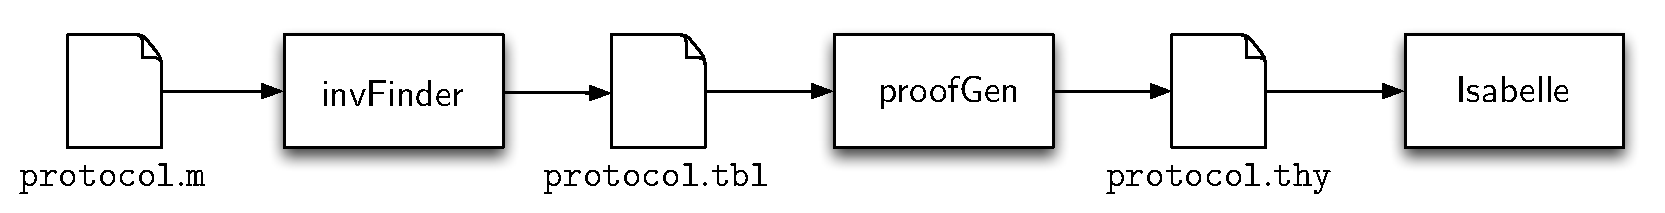
\includegraphics[width=1.0\textwidth]{paraVerifier.pdf}
\vspace{-0.6cm}
\caption{The workflow of {\sf paraVerifier}.}
\label{fig:arch}
\end{figure}


%%=========================================
%\medskip
%\noindent
%{\bf A running example.}
%%=========================================
%We present the verification of a simple cache coherence protocol {\tt mutual}
%to illustrate the functionalities of {\sf paraVerifier}.
%We need to write the protocol model in our modeling language below:
%
%\vspace{2mm}
%\begin{specification}\label{spec1}
%1\twoSpaces   pIni  N $\equiv$
%   x=true $\wedge$ (forallForm N ($\lambda$ i. n[i]=I))\\
%
%~2\twoSpaces    try i $\equiv$ n[i] = I $\vartriangleright$ n[i] := T; \\
%
%~3\twoSpaces    crit i $\equiv$ n[i] = T\& x = true $\vartriangleright$  n[i] := C; x := false;  ;\\
%
%~4\twoSpaces   exit i $\equiv$ n[i] = C $\vartriangleright$ n[i] := E; \\
%
%~5\twoSpaces   idle  i $\equiv$  n[i] = E $\vartriangleright$ n[i] := I;  x := true;\\
%
%~6\twoSpaces   prules  = [(``crit", crit), (``exit", exit), ("idle",idle),("try",try)]\\
%
%~7\twoSpaces inv1 i j $\equiv$ $\neg$ (n[i]= C $\wedge$ n[j]= C)\\
%
%~8\twoSpaces  search prules 3 [inv1 1 2] "mutual" \\
%
%~9\twoSpaces  createIsabelleModel pIni "mutual"
%\end{specification}
%%
%\noindent
%Line 1 specifies the initial states of the protocol;
%lines 2-5 describe four transition rules;
%line 6 states the set of all protocol rules and names them;
%line 7 defines the mutual exclusion property;
%line 8 is a command to invoke {\sf invFinder} to search for auxiliary invariants
%from a reference instance with 3 nodes,
%the starting invariant is the property itself, and the results are stored in a file ``{\tt mutual}";
%line 9 is a command to invoke {\sf proofGen}
%to generate a parameterized Isabelle proof script.

Starting from a given set of initial invariants,
{\sf invFinder} repeatedly tries to find new invariants,
in the form of ground formulas,
by constructing the causal relation between
the invariants and the protocol rules.
It uses an oracle\footnote{Implemented with NuSMV and the SMT solver Z3.} that checks whether a ground formula
is an invariant in the small reference model of the protocol.
{\sf invFinder} stops until no new invariants can be found.
The output of {\sf invFinder} is stored in file {\tt protocol.tbl}.
Each line of the table records
the index of an invariant,
the name of a parameterized rule,
the rule parameters to instantiate the rule,
a causal relation between the invariant and a causal relation
The table also records the proper formulas $f'$
which is used to construct the third causal relation $\mathsf{invHoldForRule}_3$.
An example of such table is shown in Tab.~\ref{label-ground-causal relation}.

%The output of {\sf invFinder}, stored in file {\tt mutual.tbl},
%is partly shown in Tab.~\ref{label-ground-causal relation}.
%Each line records
%the index of an invariant,
%the name of a parameterized rule,
%the rule parameters to instantiate the rule,
%a causal relation between the invariant and a causal relation
%The table also records the proper formulas $f'$
%which is used to construct the third causal relation $\mathsf{invHoldForRule}_3$.
%The auxiliary invariants found by {\sf invFinder} include:
%$\mathsf{inv_2}  \equiv  \neg (x=true  \wedge  n[1]=C)$, $\mathsf{inv_3}    \equiv \neg  ( n[1]=C \wedge n[2]=E)$,
%$\mathsf{inv_4}  \equiv  \neg (x=true  \wedge  n[1]=E)$,   $\mathsf{inv_5}    \equiv \neg  ( n[1]=C \wedge n[2]=C)$.

\begin{table}[!t]
\centering
\caption{An example fragment of {\tt protocol.tbl} generated by {\sf invFinder}.}\label{label-ground-causal relation}
\vspace{-2mm}
\begin{tabular}{|c|c|c|c|c|  }
\hline
protocol rule& ruleParas &~~invariant~~&~~~~causal relation~~~~&  formula ($f'$)  \\
\hline\hline
%  .. & ..&.. &..&.. \\
%\hline
  crit  & [1]& inv1 1 2& invHoldForRule3 &inv2~2 \\
\hline
  crit &[2]& inv1 1 2& invHoldForRule3 &inv2~1  \\
\hline
  crit & [3]& inv1 1 2 & invHoldForRule2  & \\
%\hline
%  .. & ..&.. &..&.. \\
\hline
\end{tabular}
\vspace{-4mm}
\end{table}

The formal Isabelle proof script {\tt protoocl.thy} generated by {\sf proofGen}
includes the definitions of control signals, rules, invariants, initializing formula,
lemmas and their proofs.
%
%Some main definitions and lemmas in {\tt mutual.thy} are listed below.
%\vspace{-2mm}
%\begin{specification} \label{spec2}
%1\twoSpaces pIniN  N $\equiv$  andList [ iniStateSpecOfx ,   iniStateSpecOfn N ]\\
%
%~2\twoSpaces
%prules N $\equiv$ \{r. ex1P N ($\lambda$i.  r=crit i)  $\vee$
%ex1P N ($\lambda$i.  r=exit i)  $\vee$\\
%\twoSpaces\twoSpaces ex1P N ($\lambda$i.  r=idle i)  $\vee$
%ex1P N ($\lambda$i.  r=try i)  \}\\
%
%~3\twoSpaces
%invariants N $\equiv$ \{f. ex2P N ($\lambda$ i j.  f = inv1 i j)  $\vee$ \\
%\twoSpaces\twoSpaces ex1P N ($\lambda$ i.  f= inv2 i)  $\vee$
%ex2P N ($\lambda$ i j.  f = inv3 i j)  $\vee$ \\
%\twoSpaces\twoSpaces ex1P N ($\lambda$ i.  f= inv4 i)  $\vee$
%ex2P N ($\lambda$ i j.  f = inv5 i j)   \}\\
%
%~4\twoSpaces lemma initImpInv1:
%    $\isasymlbrakk$ i1 $\le$ N; i2 $\le$ N;
%i1$\neq$i2; $\mathsf{formEval}$~(pIni~N)~s
%    $\isasymrbrakk$ \\
%\twoSpaces\twoSpaces $\Longrightarrow$
%invHoldForRule' (inv1  i1 i2 ) (crit iR1 ) (invariants   N)
% % (is $\forall$s. ?P1 s$\vee$?P2 s$\vee$?P3 s
%)\\
%
%~5\twoSpaces lemma critVsInv1: $\isasymlbrakk$ iR1 $\le$ N; i1 $\le$ N; i2 $\le$ N; i1$\neq$i2
%    $\isasymrbrakk$ \\
%\twoSpaces\twoSpaces $\Longrightarrow$
%invHoldForRule' (inv1  i1 i2 ) (crit iR1 ) (invariants   N)
%)\\
%
%~6\twoSpaces lemma main: $\isasymlbrakk$ s $\in$ reachableSet { pIni  N} (rules N); 0<N $\isasymrbrakk$ \\
%\twoSpaces\twoSpaces $\Longrightarrow$
%$\forall$inv. inv $\in$(invariants N)$\longrightarrow$
%formEval inv s
%\end{specification}
%
%\noindent
%Line 1 defines the specification formula of a paramaterized instance with $N$ nodes;
%line 2 lists  all the rules;
%line 3 lists all the invariant formulas;
%line 4 specifies a lemma that
%if the initial specification formula is evaluated true at a state $s$,
%then invariant formula {\tt invariants} is evaluated true at $s$ as well;
%line 5 states a lemma that the causal relation holds between rule {\tt crit} and invariant {\tt inv1};
%line 6 specifies the main lemma that  for all invariants ${\it inv}$ and for all reachable state $s$,
%${\it inv}$ is evaluated to be true at state $s$.
%
Here, we briefly explain the generalization principle involved in {\sf proofGen}.
For a ground invariant ${\it inv} $with parameters,
{\sf proofGen} analyzes the number of ground parameters in it
and defines a parameterized invariant ${\it pInv}$
by replacing the ground parameters with their corresponding symbolic parameters accordingly.
Then {\sf proofGen} explores symmetry relations
and uses the following three relations ${\sf ex1P}$ or ${\sf ex2p}$ or ${\sf ex3P}$ to define all the actually parameterized
invariants, where $\mathsf{ex1P}~ N~ P \equiv \exists i. (i \le N \wedge P~
i)$, $\mathsf{ex2P}~ N~ P \equiv \exists i~j. (i \le N \wedge j \le
N \wedge i\ne j \wedge P~ i~j)$, and $\mathsf{ex3P}~ N~ P \equiv
\exists i~j~k. (i \le N \wedge j \le N \wedge k \le N\wedge i\ne j
\wedge i\ne k \wedge j\ne k \wedge P~ i~j~k)$.
For instance, for the formula $\neg  ( n[1]=C \wedge n[2]=C)$,
two ground parameters 1 and 2 are extracted, and
a formal invariant formula $inv_1~i1~i2=\neg  ( n[i1]=C \wedge n[i2]=C)$
is defined by replacing 1 and 2 with symbolic parameters $i1$ and $i2$,
and $\{f.\mathsf{ex2P}~ N~ \lambda i1 i2. f= inv_1~i1~i2\}$ defines the set of  all the formulas, each of which is symmetric to $inv_1~1~2$.
The generalization of statements, rules, and causal relations can be defined accordingly.
Each line in the ground causal relation table (Tab.~\ref{label-ground-causal relation}),
is generalized into a parameterized relation,
which is the key to generate a proof command to select a proper causal relation to prove.

%=========================================
\section{Validation and Conclusion}
%=========================================
We implemented {\sf paraVerifier} in Forte~\cite{forte}
and tested it on a number of cache coherence protocols.
The detailed source codes and data can
be found in~\cite{LiCache14}. Each experimental data includes the
protocol model, the invariant sets, and the Isabelle proof script.
Tab.~\ref{Summarization of experiment results}
summarizes our verification results, recording
the resources needed to compute the invariants and generate the proof scripts.
Note that our proof of Flash is different from the one of Park et al.~\cite{Park1996a},
where they need to manually construct an abstract transaction model of Flash.
Our proof does not require this step and has less human interaction.

\begin{table}[!t] \label{Summarization of experiment results}
\centering
\caption{Verification results on benchmarks.}
\vspace{-2mm}
\begin{tabular}{|c|r|r|r|r|}
\hline
Protocols &  \#rules & \#invariants & time (seconds) & Memory (MB) \\
\hline\hline
MESI & 4& 3 & 0.68 & 11.5  \\
\hline
MOESI &  5& 3 &0.65 & 23.2  \\
\hline
Germanish~\cite{cubicle2011}  & 6&3&0.68 & 23.0   \\
\hline
German~\cite{Chou2004} & 13 & 24 & 4.09 & 26.7   \\
\hline
German with data~\cite{Chou2004} & 15 & 50 & 12.05 & 29.4   \\
\hline
Flash~\cite{Park1996a,McMillan2001} & 73 & 112 & 1457.42 & 169.4   \\
\hline
\end{tabular}
\vspace{-5mm}
\end{table}

%%=========================================
%\section{Conclusion}
%%=========================================
Within {\sf paraVerifier},
our automatic framework for parameterized verification of cache coherence protocol,
(1) instead of directly proving the invariants of a protocol by induction, we propose a general
proof method based on the consistency lemma to decompose the proof goal into a number of small ones;
(2) instead of proving the decomposed subgoals by hand,
we automatically generate proofs for them based on the information computed in a small protocol instance.\footnote{Technical details
of {\sf paraVerifier} will be made available in a technical report.}

As we demonstrate in this work, combining theorem proving with
automatic proof generation is promising in the field of formal
verification of industrial protocols. Theorem proving can guarantee the rigorousness of the verification results,
while automatic proof generation can release the burden of human interaction.

\paragraph*{Acknowledgments} %Yongjian Li, was supported by  grants 61170073 and  61170304 and 2011DFG13000 from the National Natural Science Foundation of China.
This work is partially supported by the National Natural Science Foundation of China under Grants No.61170073, No.61170304, No.2011DFG13000, No.61272135, No.61173007, and No.61332009.

%=========================================
%\bibliographystyle{splncsnat}
%\bibliography{gste,cache,refer}
%=========================================
\vspace{-0.5cm}
\begin{thebibliography}{10}

\bibitem{Pnueli1996}
Pnueli, A., Shahar, E.:
\newblock A platform for combining deductive with algorithmic verification.
\newblock In Porc.\ 16th Conference on Computer Aided Verification (CAV). LNCS 1102.
\newblock Springer (1996)  184--195

\bibitem{Bjorner1997}
Bj\"orner, N., Browne, A., Manna, Z.:
\newblock Automatic generation of invariants and intermediate assertions.
\newblock Theoretical Computer Science \textbf{173}(1) (1997)  49 -- 87

\bibitem{Arons2001}
Arons, T., Pnueli, A., Ruah, S., Xu, Y., Zuck, L.:
\newblock Parameterized verification with automatically computed inductive
  assertions?
\newblock In: Proc.\ 13th Conference on Computer Aided
  Verification (CAV). LNCS 2102.
\newblock Springer (2001)  221--234

\bibitem{Pnueli2001}
Pnueli, A., Ruah, S., Zuck, L.:
\newblock Automatic deductive verification with invisible invariants.
\newblock In: Proc.\ 7th Conference on Tools and Algorithms for the
  Construction and Analysis of Systems (TACAS). LNCS 2031.
\newblock Springer (2001)  82--97

\bibitem{Tiwari2001}
Tiwari, A., Rue\ss, H., Sa\"idi, H., Shankar, N.:
\newblock A technique for invariant generation.
\newblock In: Proc.\ 7th Conference on Tools and Algorithms for
  the Construction and Analysis of Systems (TACAS). LNCS 2031.
\newblock Springer (2001)  113--127

\bibitem{Chou2004}
Chou, C.T., Mannava, P., Park, S.:
\newblock A simple method for parameterized verification of cache coherence
  protocols.
\newblock In: Proc.\ 5th Conference on Formal Methods in
  Computer-Aided Design (FMCAD). LNCS 3312.
\newblock Springer (2004)  382--398

\bibitem{PFHV07}
Pang, J., Fokkink, W., Hofman, R., Veldema, R.:
\newblock Model checking a cache coherence protocol of a Java DSM implementation.
\newblock Journal of Logic and Algebraic Programming \textbf{71}(1) (2007)  1 -- 43

\bibitem{Pandav2005}
Pandav, S., Slind, K., Gopalakrishnan, G.:
\newblock Counterexample guided invariant discovery for parameterized cache
  coherence verification.
\newblock In: Proc.\ 13th IFIP Advanced Research Working Conference on Correct
  Hardware Design and Verification Methods (CHARME). LNCS 3725.
\newblock Springer (2005)  317--331

\bibitem{Lv2007}
Lv, Y., Lin, H., Pan, H.:
\newblock Computing invariants for parameter abstraction.
\newblock In: Proc.\ 5th IEEE/ACM Conference on Formal
  Methods and Models for Codesign (MEMOCODE). IEEE CS (2007)  29--38

\bibitem{Bingham2008}
Bingham B.:
\newblock Automatic non-interference lemmas for parameterized model checking.
\newblock In Proc.\ 8th Conference on Formal Methods in Computer-Aided Design (FMCAD).
\newblock IEEE CS (2008)  1--8

\bibitem{cubicle2011}
Conchon, S., Goel, A., Krstic, S., Mebsout, A., Za\"idi, F.:
\newblock Cubicle: A parallel SMT-based model checker for parameterized
  systems.
\newblock In Proc.\ 24th Conference on Computer Aided Verification (CAV). LNCS 7385.
\newblock Springer (2012)  718--724

\bibitem{McMillan2001}
McMillan, K.L., Labs, C.B.:
\newblock Parameterized verification of the Flash cache coherence protocol by
  compositional model checking.
\newblock In: Proc.\ 9th IFIP Advanced Research Working Conference on Correct
  Hardware Design and Verification Methods (CHARME). LNCS 2144. Springer
  (2001)  179--195

\bibitem{NPW02}
Nipkow, T., Paulson, L.C., Wenzel, M.:
\newblock Isabelle/{HOL} - A Proof Assistant for Higher-Order Logic. Volume
  2283 of LNCS.
\newblock Springer (2002)

\bibitem{Park1996a}
Park, S., Dill, D.L.:
\newblock Verification of Flash cache coherence protocol by aggregation of
  distributed transactions.
\newblock In: Proc.\ 8th Annual ACM Symposium on Parallel
  Algorithms and Architectures (SPAA). ACM (1996)  288--296

%\bibitem{Fan2012}
%Fan, D., Zhang, H., Wang, D., Ye, X., Song, F., Li, G., Sun, N.:
%\newblock Godson-t: An efficient many-core processor exploring thread-level
%  parallelism.
%\newblock Micro, IEEE \textbf{32}(2) (2012)  38--47

\bibitem{LiCache14}
Li, Y.:
\newblock {\sf invFinder}: An invariant finder (2014)
  \url{http://lcs.ios.ac.cn/~lyj238/invFinder.html}.

\bibitem{forte}
Technical Publications and Training, Intel Corporation:
\newblock Forte/FL User Guide. 2003.

\end{thebibliography}

\end{document}
